\def\solutionMode{TRUE}%

\documentclass[11pt]{article}%
\usepackage{solutions}%
\usepackage{374}%
\usepackage{374_extra}% 

\begin{document}

\noindent\textbf{\LARGE HW{2} Solution}\\
\noindent{\textbf{\Course: \CourseName, \Semester}}
\hfill\Version{1.0}%
\\[-0.12cm]
%
\Hr%
\smallskip%

\noindent%
Submitted by:
\begin{compactitem}
    \item \textbf{$\ll$Ray Ying$\gg$}:
    \textbf{$\ll$xinruiy2$\gg$}
    \item \textbf{$\ll$Aditya Pillai$\gg$}:
    \textbf{$\ll$apillai4$\gg$}
\end{compactitem}
\Hr
\medskip
\SaveIndent%

\begin{questions}[1]
    \item \begin{enumerate}
    \item   I choose python to implement the counters. Given a list of items, integers in my case, and count the length of the list. Whenever a new integer comes, I randomly select $1$ number from a list from $0$ to $2^{X}$ or $(1+a)^{X}$, only increases the counter $X$ when the number selected is $0$.\\
    I made $8$ copies , $a = 3$,  $\epsilon = 1/2$, and $\delta = 1/8$. 
    \item The plot of $n = 2^{16}$ to the three counters(I did eight times corresponding to the $x$ axis):\\
    \\
    \begin{figure}[h]
    \centering
    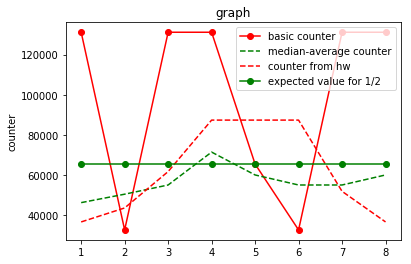
\includegraphics[width=1\textwidth]{hw2/counters.png}
    \caption{n and three counters}
    \end{figure}
    \newpage
    The plot of $n$ comparing to the needed bits($x$ is the log of the length of the array):\\
    \begin{figure}[h]
    \centering
    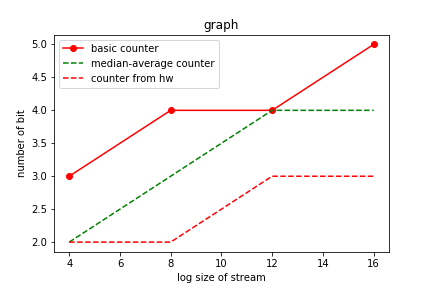
\includegraphics[width=1\textwidth]{hw2/pic.png}
    \caption{n with the bit needed}
    \end{figure}
    \\
    \item Comparing to the theoretical space, my implementation will need extra space for the step of "flip biased coins", an array of size of minimum $2^X$ or $(1+a)^{X}$ for it. Also, my code didn't implement a bit counter. \\
    The performance is pretty accurate to the expectation, when doing the basic counter, the value is pretty inaccurate due to the large variance. After doing the average and median trick, the expected success rate that the value is in the range of $\epsilon = 1/2$ times the length of the array should be $1- \delta = 7/8$ and the success rate in my experiment is just $7/8$. When I use the way describe in the homework, the number of bits required reduce but it seems less reliable than using $(1/2^x)$ rather than $1/(1+a)^x$ with higher variance.\\
    Also, when given the string length too big, the computer is really hard and slow at computing the counter especially with average and median tricks. 
    
    \end{enumerate}
    \\
    \item  Let $X_i$ be 1 if $h(b_i) \leq n/2^{i-2}$, and let $X = \sum_{i=1}^{d}X_i$. \\
    $\mathbb{E}(X_i) = 1/2^{i-2}$ and $\mathbb{E}(X) = d/2^{i-2}$ by linearity of expectation.\\
    $\mathrm{Var}(X_i) = \frac{1}{2^{i-2}}(1 - 1/2^{i-2})$,  $\mathrm{Var}(X) = \frac{d}{2^{i-2}}(1 - 1/2^{i-2})$, since we have pairwise independence. \\ 
    \\
    To use Chebyshev, we find the probability that $X - \mathbb{E}(X) \leq - \mathbb{E}(X) \implies |X - \mathbb{E}(X)| \geq  \mathbb{E}(X) $ because this implies that $X \leq 0$. \\
    
    $\Pr(X \leq 0 ) \leq \Pr[|X - \mathbb{E}(X)| \geq d/2^{i-2}] \leq \frac{\frac{d}{2^{i-2}}(1 - 1/2^{i-2})}{d^2/(2^{i-2})^2} = \frac{(1 - 1/2^{i-2})}{ d/2^{i-2}} < \frac{1}{d/2^{i-2}} < \frac{1}{2} $\\
    \\
    The expected balls falls in the range of $[1,\frac{n}{2^{i+3}})$ is $d \cdot \frac{\frac{n}{2^{i+3}}}{n}$, let $X'$ be the number of balls fall in the range of $[1,\frac{n}{2^{i+3}})$, by Markov inequality, we can have $Pr[X' \geq 1] \leq d \cdot \frac{\frac{n}{2^{i+3}}}{n}$, therefore, $Pr[X' = 0] \geq 1 - d \cdot \frac{\frac{n}{2^{i+3}}}{n} \geq \frac{3}{4}$ as $d \in [2^i, 2^{i+1})$.\\
    \\
    It's lower bound for $Pr[X'=0]$ and it's upper bound for $Pr[X=0]$, therefore, we can get a lower bound for the difference. Hence, $Pr[Z \in [n/2^{i+3}, n/2^{i-2})] = Pr[X' = 0] - Pr[X = 0] > 1/4$.
    \\
    \item
    \begin{enumerate}
    \item  $\Pr(Z = 1) = \lceil (1 - \epsilon)t / d \rceil$ 
    \item Let $X_{j | i}$ be the indicator that $h(b_j) \leq (1 - \epsilon)tN / d \rceil$ conditioned on $Z = 1$ \\
    $\mathrm{Var}(X_j) = \frac{(1 - \epsilon)t}{d}(1 - (1 -  \epsilon)t / d)$ \\
    Let $X = \sum_{i= 1}^{d-1} X_i$, then $\mathbb{E}(X) = (1 - \epsilon)t(d-1)/d \leq (1 - \epsilon)t$ $\mathrm{Var}(X) = d - l \mathrm{Var}(X_j)$ the variances can be added since the hash function is $3$-wise independent, $2$ conditioning on $Z = 1$ makes the $X_j$ variables pairwise independent so the variances can be added. \\
    \begin{align*}
        \Pr(X \geq t) &\leq Pr(|X - \mathbb{E}(X)| \geq t - \mathbb{E}(X)) \\
        &\leq Pr(|X - \mathbb{E}(X)| \geq t\epsilon)\\
        & \leq \mathrm{Var}(X)/\epsilon^2 t^2 \\
        & \leq (1 - \epsilon)t/\epsilon^2 t^2 \\
        &= (1 - \epsilon)\epsilon \\
        &\leq (1 + \epsilon)\epsilon
    \end{align*}
    \item $\Pr(h(b_i) = h(b_j)) = N/N^2 = 1/n^3$ \\
    By union bound the probability of a collision with $h(b_i)$ is at most $\frac{d-1}{n^3} \leq 1/n^2 \leq 1/tn \leq \epsilon^3/n \leq \epsilon t/n \leq t\epsilon/d$ 
    \item The probability that $b_i$ is outputted is at least the probability the event 1 in part 1 occurred, at most $t-1$ other elements landed in the same range as $b_i$, and no elements collided with $b_i$. Let these events be $A, B,C$ respectively. \\
    \begin{align*}
        \Pr(A \cap B \cap C) &= \Pr(A) \Pr(B | A) \Pr(C | A, B) \\
        &\geq \frac{(1- \epsilon)t}{d} (1 - \epsilon(1 + \epsilon))\Pr(C | A, B) \\
         &\geq \frac{(1- \epsilon)t}{d} (1 - \epsilon(1 + \epsilon))(1 - t\epsilon/d) \tag{3 gives upper bound on the complement of $C | A, B$} \\
         &\geq \frac{(1- \epsilon)t}{d} (1 - \epsilon(1 + \epsilon))(1 - \epsilon) \\
         &= \frac{(1- \epsilon)t}{d} (1 - 2 \epsilon + \epsilon^3) \\
         &\geq \frac{(1- \epsilon)t}{d} \epsilon^3 \tag{$\epsilon$ < 1/2} \\
         &= \frac{(1- \epsilon)}{d} \\
         &\geq \frac{1 - 10 \epsilon}{d}
    \end{align*}
    \end{enumerate}
    \\
    \item
    \\
    \begin{enumerate}
    \\
    \item  
    \begin{align*}
        e \sum_{i = 1}^{n} g(f_i) &= e \sum \frac{f_i}{em} \ln(\frac{me}{f_i}) \\
        &= e\sum \frac{f_i}{em} (\ln(\frac{m}{f_i}) + 1) \\
        &= e(\sum \frac{f_i}{em} \ln(\frac{m}{f_i}) + \sum \frac{f_i}{em}) \\
        &= e(\frac{1}{e} \sum \frac{f_i}{m} \ln(\frac{m}{f_i}) + \frac{1}{e}) \\
        &= \Phi + 1
    \end{align*}
    \item
    $\frac{d}{dl}(g(\ell)) = \frac{m}{e}\log(\frac{m}{\ell}) > 0$ when $\ell \leq m$ so $g(\ell)$ is increasing and $g(\ell) \geq g(\ell - 1)$
    \item 
    \begin{align*}
        g(\ell) - g(\ell - 1) &= \frac{\ell}{em}\ln(\frac{me}{\ell}) - \frac{\ell - 1}{em}\ln(\frac{me}{\ell - 1}) \\
        &= \frac{\ell}{m}(\ln(m) + 1 -\ln(\ell)) - \frac{\ell - 1}{em}(\ln(m) + 1 - \ln(\ell - 1)) \\
        &= \frac{\ln(m) + 1}{em} - \frac{\ell \ln(m)}{em} + \frac{(\ell - 1)\ln(\ell -1)}{em} \\
        &\leq \frac{\ln(m) + 1}{em}
    \end{align*}
    \item
    \begin{align*}
        \mathrm{Var}[Y] \leq \mathbb{E}[Y^2] &= \sum \frac{f_i}{m} \sum_{\ell = 1}^{f_i}\frac{m^2}{f_i}(g(\ell) - g(\ell - 1))^2 \\
        &\leq \frac{1 + \ln(m)}{e} \sum \sum_{\ell = 1}^{f_i}g(\ell) - g(\ell - 1) \\
        &= \frac{1 + \ln(m)}{e} \sum g(f_i) \\
        &= \frac{1 + \ln(m)}{e^2} (1 + \Phi)
    \end{align*}
    $c_1 = 1/e^2$
    \item Since we made $t$ parallel copy of the algorithm, the variance will reduced to $1/t$ to the original. Also, we are not calculating variance on $Y$ but $eY$, $Var(eY) = e^2\cdot Var(Y)$. Since we proved in the last step that the original $Var(Y)\leq \frac{1}{e}\cdot (1+ \ln(m))E[Y]$, the new variance will be 
    $$Var(Y') \leq \frac{e\cdot (1+ \ln(m))E[Y]}{t} = \frac{e\cdot (1+ \ln(m))E[Y]}{c(1+ \ln(m))/\epsilon^2} = \frac{\epsilon^2(1+\phi)}{c}$$
    Now, by chebyshev's inequality,
    $$ P[|eZ - (1+\phi)|\geq \epsilon(1+\phi)] \leq \frac{Var(Y')}{\epsilon^2(1+\phi)^2} = \frac{1}{c(1+\phi)}$$
    We want to show that $\frac{1}{c(1+\phi)} \leq \frac{1}{4} \implies \frac{4}{1+\phi}\leq c$. It's easy to see that $1+\phi \geq 1$ since the length of the stream is at least $1$, $c \geq 4$.
    \item We create the $8\ln(1/\delta)$ copy of part $5$, let's make an indicator $Z$, for each copy, if the average result is in the range of $(1\pm \epsilon)(1 + \phi)$, then we add $1$ to the $Z$, otherwise, we add $-1$ to the $Z$. Let $k = 8\ln(1/\delta)$, the $E[Z] = \frac{k}{4}\times(-1) + \frac{3k}{4}\times(1) = \frac{k}{2}$.\\
    Since if the median is bad, half of the copies are bad, then $E[Z] \leq 0$. We applied to Chernoff's bound:\\
    $$Pr[|Z-E[Z]| \geq \abs{(\frac{k}{2} - 0)}] = Pr[|Z-E[Z]| \geq \frac{k}{2}] \leq 2\cdot e^{\frac{-(\frac{k}{2})^2}{2k}} = 2\cdot e^{-\frac{k}{8}} = 2 \cdot \delta$$
    Then the probability of having a bad median is less than $2 \cdot \delta /2 = \delta$ because we take the absolute value of $Z-E[Z]$, the probability of $Z \geq E[Z]$ and $Z - E[Z] \geq \frac{k}{2}$ is the same to the probability of $Z \leq E[Z]$ and $ E[Z] - Z \geq \frac{k}{2}$.\\ Therefore, we use $O(8\ln(1/\delta)ln(m)/\epsilon^2) = O(\ln(1/\delta)ln(m)/\epsilon^2)$ independent samples to get a result within $(1+\epsilon)$ with probabilty $\geq 1-\delta$.
    \end{enumerate}
\end{questions}


\end{document}

%%%%%%%%%%%%%%%%%%%%%%%%%%%%%%%%%%%%%%%%%%%%%%%%%%%%%%%%%%%%%%%%%%%%%%%%
%%%%%%%%%%%%%%%%%%%%%%%%%%%%%%%%%%%%%%%%%%%%%%%%%%%%%%%%%%%%%%%%%%%%%%%%
%%%%%%%%%%%%%%%%%%%%%%%%%%%%%%%%%%%%%%%%%%%%%%%%%%%%%%%%%%%%%%%%%%%%%%%%
